\documentclass{article}

\usepackage{geometry}
\usepackage{amsmath}
\usepackage{graphicx}
\usepackage{listings}
\usepackage{xcolor}
\usepackage{chngcntr}


\geometry{letterpaper, margin=1.5in, bottom=1in}

\counterwithin*{equation}{subsection}

\title{Problem Set Three}
\date{03/20/2018}
\author{Zhixian(Jason) Yu}

\definecolor{mygreen}{rgb}{0,0.6,0}
\definecolor{mygray}{rgb}{0.9,0.9,0.9}
\definecolor{mymauve}{rgb}{0.58,0,0.82}

\lstset{ %
  backgroundcolor=\color{mygray},   % choose the background color
  basicstyle=\footnotesize,        % size of fonts used for the code
  breaklines=true,                 % automatic line breaking only at whitespace
  captionpos=b,                    % sets the caption-position to bottom
  commentstyle=\color{mygreen},    % comment style
  escapeinside={\%*}{*)},          % if you want to add LaTeX within your code
  keywordstyle=\color{blue},       % keyword style
  stringstyle=\color{mymauve},     % string literal style
  keepspaces=true,
  tabsize=2,
  language=Python,
  numbersep=3pt, 
  numbers=left
  %frame=single
}

\begin{document}
\maketitle
\pagenumbering{gobble}
\newpage

\section{Theory}
\subsection*{Problem 1/3}
Because $u$ and $v$ are unit vectors, the cosine of the angle between $u$ and $v$ is:
\begin{equation}
cos\theta = u^T v
\end{equation}
We can get a necessary condition by taking the partial derivatives over $u, v$ and set them to zero. Thus we get:
\begin{align}
\frac{\partial A}{\partial u} &= Av - 2\lambda u = 0 \\
\frac{\partial A}{\partial v} &= (u^TA)^T - 2\mu v = 0
\end{align}
We can rewrite the above equation and get:
\begin{align}
Av &= 2\lambda u  \label{eq:dAdu}\\
u^TA &= 2\mu v^T \label{eq:dAdv}
\end{align}
Because $u^Tu=1$, we get the following if we multiply equation~\ref{eq:dAdu} by $u^T$ from the left:
\begin{equation}
\label{eq:2lambda}
u^TAv = 2\lambda u^Tu = 2\lambda
\end{equation}
Similarly because $v^Tv=1$, we get from equation~\ref{eq:dAdv}
\begin{equation}
\label{eq:2mu}
u^TAv = 2\mu v^Tv = 2\mu
\end{equation}
From equations~\ref{eq:2lambda} and \ref{eq:2mu}, we get $\lambda=\mu$. Let $\sigma=2\lambda$, equations~\ref{eq:dAdu} and \ref{eq:dAdv} become:
\begin{align*}
Av &= \sigma u \\
A^T u &= \sigma v
\end{align*}
Because $u$ and $v$ are unit-length vectors, $\sigma$ is a singular value for A, and $u, v$ are the left-singular and right-singular vectors, respectively. Thus the necessary condition for the solution is given by SVD, i.e. $A=u\sigma v^T$.

\subsection*{Problem 2}
\paragraph{a)} Let $P=\frac{1}{n}ee^T$, so:
\begin{align*}
P^2 &= \frac{1}{n^2}ee^Tee^T
\end{align*}
Since $e^Te=n$, we have:
\begin{align*}
P^2 &= \frac{1}{n^2}ene^T \\
&= \frac{1}{n}ee^T \\
&= P
\end{align*}
Therefore $\frac{1}{n}ee^T$ is a projection. 
\paragraph{b)}
The projection first calculates the mean point of the set of points, and then projects each of the point to the same mean point. 
\paragraph{c)}
By applying the $H$ matrix from the left, we have:
\begin{equation*}
B = HA = A - \frac{1}{n}ee^TA
\end{equation*}
Suppose $a_{ij}$ and $b_{ij}$ are the ith row, jth column elements of A and B, respectively. So:
\begin{align*}
b_{ij} &= a_{ij} - \frac{1}{n}\sum_{k=1}^{n}(1\cdot a_{kj}) \\
&=a_{ij} - \frac{1}{n}\sum_{k=1}^{n}a_{kj}
\end{align*}
Therefore it subtracts each element $a_{ij}$ of A by the mean value of the jth column elements. In addition, each column of $B$ has a sum of 0, showing in the following:
\begin{align*}
\sum_{l=1}^{n}b_{lj} &= \sum_{l=1}^{n}(a_{lj}  - \frac{1}{n}\sum_{k=1}^{n}a_{kj}) \\
&= \sum_{l=1}^{n}a_{lj} - n(\frac{1}{n}\sum_{k=1}^{n}a_{kj})\\
&= \sum_{l=1}^{n}a_{lj} - \sum_{k=1}^{n}a_{kj}\\
&=0, \forall j \in [1,n]
\end{align*}
\paragraph{d)}
Similarly with last problem
\begin{equation*}
B = AH = A - \frac{1}{n}Aee^T
\end{equation*}
Suppose $a_{ij}$ and $b_{ij}$ are the ith row, jth column elements of A and B, respectively. So:
\begin{align*}
b_{ij} &= a_{ij} - \frac{1}{n}\sum_{k=1}^{n}(a_{ik}\cdot 1) \\
&=a_{ij} - \frac{1}{n}\sum_{k=1}^{n}a_{ik}
\end{align*}
Therefore it subtracts each element $a_{ij}$ of A by the mean value of the ith row elements. Similarly, the row sum of the result matrix $B$ is 0. 
\begin{align*}
\sum_{l=1}^{n}b_{il} &= \sum_{l=1}^{n}(a_{il}  - \frac{1}{n}\sum_{k=1}^{n}a_{ik}) \\
&= \sum_{l=1}^{n}a_{il} - n(\frac{1}{n}\sum_{k=1}^{n}a_{ik})\\
&= \sum_{l=1}^{n}a_{il} - \sum_{k=1}^{n}a_{ik}\\
&=0, \forall i \in [1,n]
\end{align*}
\paragraph{e)}
We need to show that applying $H$ from the right does not change the column sum of $HA$, i.e. 0. If we expand $B=HAH$, we get:
\begin{align*}
\label{2e_first_eq}
b_{ij} &= (HA)_{ij} - \frac{1}{n}(HAee^T)_{ij}
\end{align*}
and we want to prove
\begin{equation*}
\sum_{l=1}^{n}b_{lj} = 0
\end{equation*}
As was shown in problem \textbf{c)}, $\sum_{l=1}^{n}(HA)_{lj} = 0, \forall j \in [1,n]$. therefore:
\begin{align*}
\sum_{l=1}^{n}b_{lj} &= \sum_{l=1}^{n}(HA)_{lj} - \frac{1}{n}\sum_{l=1}^{n}(HAee^T)_{lj} \\
&= - \frac{1}{n}\sum_{l=1}^{n}(HAee^T)_{lj}\\
&= - \frac{1}{n}\sum_{l=1}^{n}\sum_{k=1}^{n}[(HA)_{lk} \cdot 1]\\
&= - \frac{1}{n}\sum_{l=1}^{n}\sum_{k=1}^{n}(HA)_{lk} \\
&= - \frac{1}{n}\sum_{k=1}^{n}[\sum_{l=1}^{n}(HA)_{lk}] \\
&= 0, \forall j \in [1,n]
\end{align*}
Therefore, sum of any column of $B$ will be 0. 

\subsection*{Problem 3}
\label{subsec:1.3}
We have
\begin{align*}
He &= (I-ee^T/n)e \\
&= e - ee^Te/n \\
&= e - e \\
&= 0e
\end{align*}
Therefore the vector of ones is an eigenvector of B, and the associated eigenvalue is 0.

\subsection*{Problem 4}
As is shown in problem 3, $Be=0$. Therefore
\begin{align}
\label{eq:be=0}
Be = \overset{\sim}{V}(\overset{\sim}{V}^Te) = 0
\end{align}
In equation~\ref{eq:be=0}, $\overset{\sim}{V}(\overset{\sim}{V}^Te)$ means the linear combination of the columns of $\overset{\sim}{V}$ weighted by $(\overset{\sim}{V}^Te)$. Because the columns of $\overset{\sim}{V}$ are different eigenvectors associated with different eigenvalues (times different constants), the columns of $\overset{\sim}{V}$ are linearly independent. Therefore, equation~\ref{eq:be=0} only has the trivial solution, and $\overset{\sim}{V}^Te=0$. 

\subsection*{Problem 5}
In $\overset{\sim}{V}^T$, each column is a configuration. Let $a_{ij}$ be the ith row, jth column element of $\overset{\sim}{V}^T$. Because $\overset{\sim}{V}^Te=0$, we have:
\begin{align*}
\sum_{j=1}^{n}(a_{ij}\cdot 1) &= \sum_{j=1}^{n}a_{ij} \\
&=  0, \forall i \in [1,n]
\end{align*}
This means for each row, the sum across all the columns of $\overset{\sim}{V}^T$ is 0, therefore the mean of all the configurations is the origin. 

\newpage
\section{Programming}
The following code sets up the environment and import packages.
\begin{lstlisting}
	import numpy as np
	import matplotlib.pyplot as plt
\end{lstlisting}
\subsection*{Problem 1}
The following code defines a function to execute MDS algorithm.
\begin{lstlisting}
	def MDS(D):
		'''
		This function computes MDS with a distance matrix
		:param D: input distance matrix
		:return: V_tilde, whose rows are result configurations, and the eigenvalues
		'''
		P = D.shape[0]  # D is a symmetric distrance matrix
		A = -0.5 * D**2
		H = np.eye(P) - np.ones((P, P))/P
		B = H@A@H
		w, V = np.linalg.eig(B)
		V = V[:, np.flip(np.argsort(w), axis=0)]
		w = w[np.flip(np.argsort(w), axis=0)]
		V = V[:, w>0]
		w = w[w>0]
		V_tilde = V * np.sqrt(w[None, :])

        return V_tilde, w
\end{lstlisting}
We can compute city coordinates using MDS from distance matrix, as is shown below:
\begin{lstlisting}
	M = np.array([[0,244,218,284,197,312,215,469,166,212,253,270],
	[0,0,350,77,167,444,221,583,242,53,325,168],
	[0,0,0,369,347,94,150,251,116,298,57,284],
	[0,0,0,0,242,463,263,598,257,72,340,164],
	[0,0,0,0,0,441,279,598,269,170,359,277],
	[0,0,0,0,0,0,245,169,210,392,143,378],
	[0,0,0,0,0,0,0,380,55,168,117,143],
	[0,0,0,0,0,0,0,0,349,531,264,514],
	[0,0,0,0,0,0,0,0,0,190,91,173],
	[0,0,0,0,0,0,0,0,0,0,273,111],
	[0,0,0,0,0,0,0,0,0,0,0,256],
	[0,0,0,0,0,0,0,0,0,0,0,0]])
	D = M+M.T

	# compute results
	res, evals = MDS(D)

	# plot cities
	cities = ['Inverness', 'Glasgow', 'Newcastle', 'Carlisle', 'Leeds', 'Hull', 'Norwich', 'Aberystwyth', 'London', 'Dover', 'Brighton', 'Exeter']
	cities = sorted(cities)
	plt.plot(res[:, 0], res[:, 1], 'r.')
	for i in range(res.shape[0]):
		plt.text(res[i, 0]+1, res[i, 1]+1, cities[i])
	plt.show()
\end{lstlisting}
The created map is shown in figure~\ref{fig:city_map_problem1}. It is similar to the actual map of UK shown in figure~\ref{fig:uk_map}.

\begin{figure}[h!]
\centering
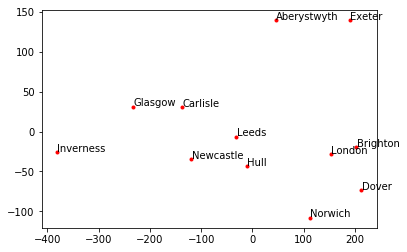
\includegraphics[width=0.6\linewidth]{../images/1.png}.
\caption{The city map based on generated coordinates.}
\label{fig:city_map_problem1}
\end{figure}
\begin{figure}[h!]
\centering
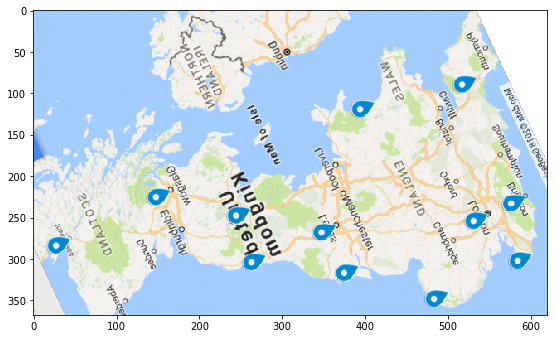
\includegraphics[width=0.6\linewidth]{../images/uk_map.png}.
\caption{An actual UK map showing cities in the problem set.}
\label{fig:uk_map}
\end{figure}

The mean of the configuration is verified to be 0.
\begin{lstlisting}
>>>print(np.mean(res, 0))
[  7.10542736e-15  -3.43428989e-14   4.26325641e-14  -5.16623781e-14
   5.53631215e-14  -2.04281037e-14   1.05545202e-13   1.95339693e-12]
\end{lstlisting}
	
We can also plot the eigenvalues of $B$ using the following code:
\begin{lstlisting}
	plt.plot(evals, '.')
	plt.show()
\end{lstlisting}
The eigenvalues is shown in figure~\ref{fig:eval}. From it we can see that the first two dimensions are already sufficient to closely approximate the point configurations. 

\begin{figure}[h!]
\centering
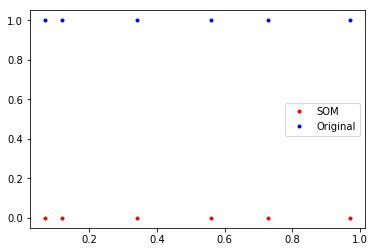
\includegraphics[width=0.6\linewidth]{../images/2.png}
\caption{The eigenvalues of B.}
\label{fig:eval}
\end{figure}

\subsection*{Problem 2}
In this problem, I removed the city Aberystwyth, and used LMDS to compute the coordinate of Aberystwyth.
The following function implements the LMDS algorithm.
\begin{lstlisting}
	def LMDS(D, dist_a, V_tilde_inv):
		'''
		:param D: the landscape marks distance matrix (not squared)
		:param dist_a: the distance vector from new point to landscape points(not squared)
		:param V_tilde_inv: the pseudo inverse of V_tilde
		:return: the configuration of the new point
		'''
		P = D.shape[0]  # dimension of data
		d_mean = (np.mean(D**2, axis= 1)).reshape(P, 1)
		d_a = (dist_a**2).reshape(P, 1)
		return -0.5*(V_tilde_inv.T@(d_a - d_mean))
\end{lstlisting}
The following code removes the city Aberystwyth and creates a new distance matrix. MDS was used to recreate the configurations based on the new distance matrix. The new map is also plotted as shown in figure~\ref{fig:new_map}. Note that in figure~\ref{fig:new_map}, blue dots were coordinates from last problem, and red dots are new coordinates computed without Aberystwyth. There are some minor differences between two sets of configurations. 
\begin{lstlisting}
	D_new = np.delete(D, [0], 0)
	D_new = np.delete(D_new, [0], 1)
	V_tilde, lamb = MDS(D_new)
	
	# plot new map
	plt.plot(V_tilde[:, 0], V_tilde[:, 1], 'r.')
	plt.plot(-res[:, 0], res[:, 1], 'b.')
	for i in range(V_tilde.shape[0]):
		plt.text(V_tilde[i, 0]+1, V_tilde[i, 1]+1, cities[i+1])
	plt.gca().invert_xaxis()
	plt.show()
\end{lstlisting}

\begin{figure}[h!]
\centering
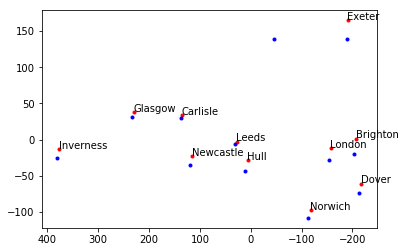
\includegraphics[width=0.6\linewidth]{../images/3.png}
\caption{New map without Aberystwyth.}
\label{fig:new_map}
\end{figure}

Now LMDS is used to compute the configuration of Aberystwyth, and plot it. 
\begin{lstlisting}
	V_tilde_inv = V_tilde / lamb[None, :]
	x_a = LMDS(D_new, D[1:, 0], V_tilde_inv)

	# plot new configuration
	plt.plot(V_tilde[:, 0], V_tilde[:, 1], 'r.')
	plt.plot(-res[:, 0], res[:, 1], 'b.')
	for i in range(V_tilde.shape[0]):
		plt.text(V_tilde[i, 0]+1, V_tilde[i, 1]+1, cities[i+1])
	plt.gca().invert_xaxis()
	plt.plot(x_a[0, 0], x_a[1, 0], 'c*')
	plt.show()
\end{lstlisting}
As is shown in figure~\ref{fig:final}, the configuration of Aberystwyth (shown as cyan star)is successfully recreated with some minor differences. 

\begin{figure}[h!]
\centering
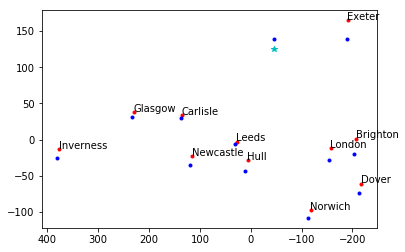
\includegraphics[width=0.6\linewidth]{../images/4.png}
\caption{Map with LMDS-recreated Aberystwyth coordinate.}
\label{fig:final}
\end{figure}
In addition, we can quantify the loss of reconstructing the configuration points with 2-dimensions using the following code. The loss is defined as $\frac{\Vert D' - D\Vert}{\Vert D \Vert}$, where $D'$ is the constructed distance matrix, and $D$ is the original matrix. MDS method has a loss of 0.051, and LMDS method has a loss of 0.061. The losses are relatively small, and MDS with all points is slightly better than LMDS which left one point out.
\begin{lstlisting}
	from scipy.spatial import distance_matrix
	D_MDS = distance_matrix(res[:,:2], res[:,:2])
	new_config = np.vstack((x_a[:2].reshape(1,2), V_tilde[:, :2]))
	D_LMDS = distance_matrix(new_config, new_config)

	print(np.linalg.norm(D_MDS-D)/np.linalg.norm(D)) #0.051
	print(np.linalg.norm(D_LMDS-D)/np.linalg.norm(D)) #0.061
\end{lstlisting}


\end{document}